% This LaTeX was auto-generated from MATLAB code.
% To make changes, update the MATLAB code and export to LaTeX again.

\documentclass{article}

\usepackage[utf8]{inputenc}
\usepackage[T1]{fontenc}
\usepackage{lmodern}
\usepackage{graphicx}
\usepackage{color}
\usepackage{hyperref}
\usepackage{amsmath}
\usepackage{amsfonts}
\usepackage{epstopdf}
\usepackage[table]{xcolor}
\usepackage{matlab}
\usepackage[active,tightpage]{preview}


\renewcommand{\PreviewBorder}{0.7in}
\newcommand{\Newpage}{\end{preview}\begin{preview}}

\sloppy
\epstopdfsetup{outdir=./}
\graphicspath{ {./assignment_2_formative_images/} }

\begin{document}
\begin{preview}

\matlabtitle{ECEN 415 Assignment 2}

\begin{par}
\begin{center}
Niels Clayton: 300437590
\end{center}
\end{par}

\matlabheading{Section A - Formative Questions}

\hrule\vspace{15pt}
\matlabheadingtwo{\textbf{Question 1.} }
\hrule\vspace{20pt}

\begin{par}
\begin{flushleft}
A state space system is described by the system matrices:
\end{flushleft}
\end{par}


\begin{matlabcode}
clc;
clear;

A = [12.5314 , -91.36 , 28.7129 , 59.9628 ; 
     21.316 , -115.6631 , 37.5584 , 75.0519 ; 
     13.967 , -53.5817 , 15.4161 , 33.4391 ; 
     20.5222 , -123.3107 , 42.267 , 79.7156];
 
B = [1.7649 , 1.7649; 
     2.8318 , 2.8318; 
     2.2353 , 2.2353; 
     2.7294 , 2.7294];
 
C = [-0.46166 , -4.4635 , 1.9151 , 3.7274 ;
     1.0853 , -12.82 , 4.5753 , 8.3759];
 
D = [0 , 0 ; 
     0 , 0 ];
\end{matlabcode}

\hrule

\matlabheadingthree{\textbf{(a)    }}

\begin{par}
\begin{flushleft}
If the system begins in a state $\mathit{\mathbf{x}}\left(0\right)={\left\lbrack 1\;\;\;\;1\;\;\;\;1\;\;\;\;2\right\rbrack }^T \;$, use matlab’s '\texttt{\textbf{lsim}}\texttt{'} command to plot the response of the system in the time interval $t\in \left\lbrack 0,10\right\rbrack s$. You should plot the evolution of the system state $\left(\mathit{\mathbf{x}}\right)$ and its output $\left(\mathit{\mathbf{y}}\right)$ as a functions of time.
\end{flushleft}
\end{par}

\begin{matlabcode}
x_0 = [1, 1, 1, 2]';     % Initial System State

sys = ss(A, B, C, D);   % Create the system

t = 0:0.001:10;         % Setup the times series
u = zeros(length(t),2); % Generate steady state input

% Run the system simulation
[y, t, x] = lsim(sys, u, t, x_0);

% Plot the state variable x
figure();
plot(t, x);
title("System State Variable x");
xlim([0.00 6.00]);
ylim([-6.0 10.0]);
legend("x_1", "x_2", "x_3", "x_4");
grid on;
\end{matlabcode}
\begin{center}
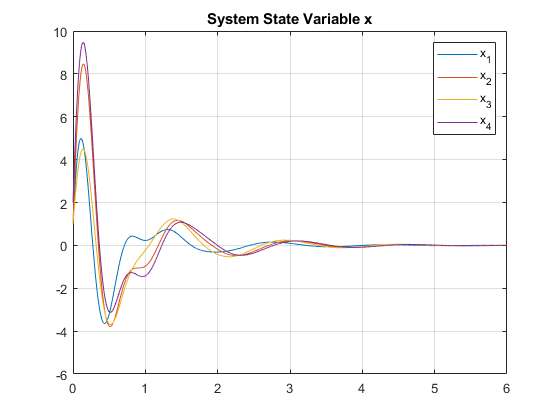
\includegraphics[width=\maxwidth{56.196688409433015em}]{figure_0.png}
\end{center}
\begin{matlabcode}
% Plot the output variable y
figure();
plot(t, y);
title("System Output Variable y");
xlim([0.00 6.00]);
ylim([-6.0 10.0]);
legend("y_1", "y_2");
grid on;
\end{matlabcode}
\begin{center}
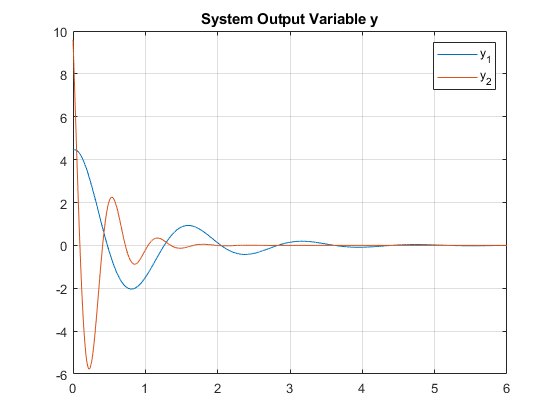
\includegraphics[width=\maxwidth{56.196688409433015em}]{figure_1.png}
\end{center}

\hrule
\matlabheadingthree{(b)}

\begin{par}
\begin{flushleft}
Replicate the results from above using the matrix exponential to evolve the state, rather than '\texttt{\textbf{lsim}}\texttt{'}
\end{flushleft}
\end{par}

\begin{matlabcode}
x_e = [];
y_e = [];

for t_ = 0:0.001:10
    xe = expm(t_*A)*x_0;
    ye = C*xe + D*[0; 0];
    
    x_e = [x_e; xe'];
    y_e = [y_e; ye'];
end

% Plot the state variable x
figure();
plot(t, x_e);
title("System State Variable x");
xlim([0.00 6.00]);
ylim([-6.0 10.0]);
legend("x_1", "x_2", "x_3", "x_4");
grid on;
\end{matlabcode}
\begin{center}
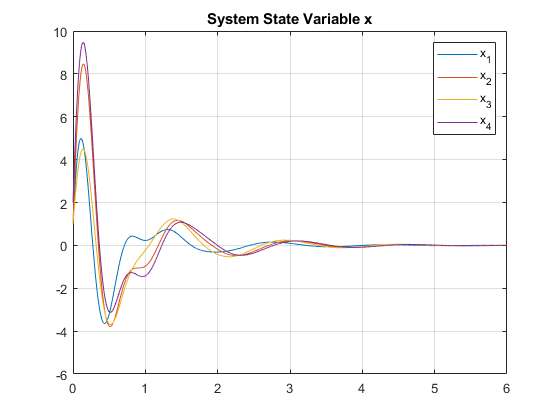
\includegraphics[width=\maxwidth{56.196688409433015em}]{figure_2.png}
\end{center}
\begin{matlabcode}
% Plot the output variable y
figure();
plot(t, y_e);
title("System Output Variable y");
xlim([0.00 6.00]);
ylim([-6.0 10.0]);
legend("y_1", "y_2");
grid on;
\end{matlabcode}
\begin{center}
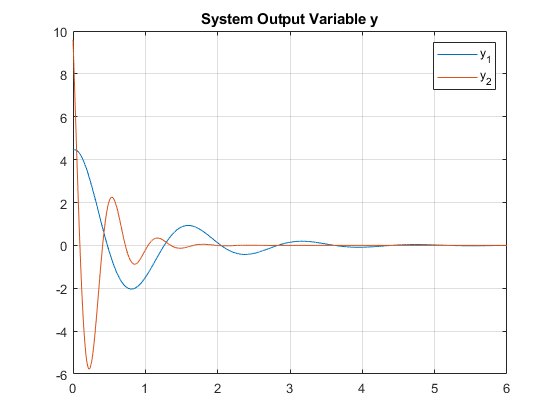
\includegraphics[width=\maxwidth{56.196688409433015em}]{figure_3.png}
\end{center}


\hrule
\matlabheadingthree{(c) }

\begin{par}
\begin{flushleft}
Use \texttt{\textbf{lsim}} to plot the response of the system to the input signal $\mathit{\mathbf{u}}={\left\lbrack u_1 \;\;\;\;u_2 \;\right\rbrack }^T$ with:
\end{flushleft}
\end{par}

\begin{par}
$$\begin{array}{l}
u_1 =u\left(t-1\right)\\
u_2 =2u\left(t-5\right)
\end{array}$$
\end{par}

\begin{par}
\begin{flushleft}
for $u$ the (Heaviside) unit step function.
\end{flushleft}
\end{par}

\begin{matlabcode}
u = zeros(length(t),2); % Generate two separate step inputs
u(t>1, 1) = 1;
u(t>5, 2) = 2;

% Run the system simulation
[y_h, t_h, x_h] = lsim(sys, u, t, x_0);

% Plot the output variable y
figure();
plot(t_h,y_h);
grid on;
title("System Output Variable y");
legend("y_1", "y_2");
\end{matlabcode}
\begin{center}
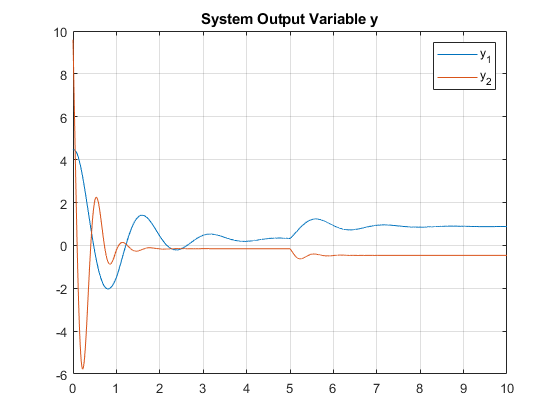
\includegraphics[width=\maxwidth{56.196688409433015em}]{figure_4.png}
\end{center}
\begin{matlabcode}
% Plot the state variable x
figure();
plot(t_h, x_h);
title("System State Variable x");
xlim([0.00 6.00]);
ylim([-6.0 10.0]);
legend("x_1", "x_2", "x_3", "x_4");
grid on;
\end{matlabcode}
\begin{center}
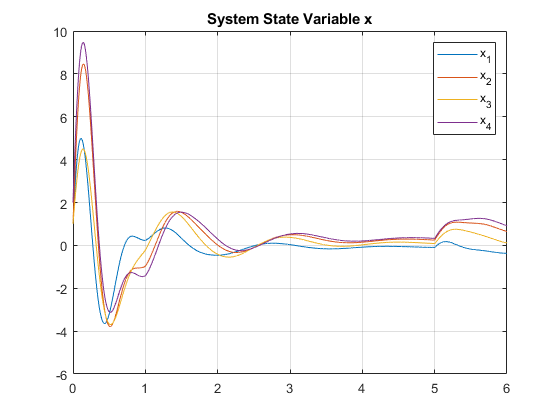
\includegraphics[width=\maxwidth{56.196688409433015em}]{figure_5.png}
\end{center}
\begin{matlabcode}
% Plot the system unput variable u
figure();
plot(t,u);
grid on;
ylim([0.00 3.00]);
title("System Input Variable u");
legend("u_1", "u_2");
\end{matlabcode}
\begin{center}
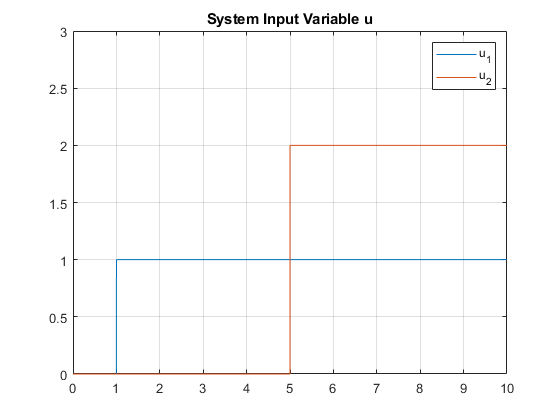
\includegraphics[width=\maxwidth{56.196688409433015em}]{figure_6.png}
\end{center}


\hrule
\matlabheadingthree{(d)}

\begin{par}
\begin{flushleft}
Use \texttt{\textbf{c2d}} to discretize the system with an appropriate sampling frequency and use \texttt{\textbf{lsim}} to plot the response of the discrete time system.
\end{flushleft}
\end{par}

\begin{matlabcode}
ts = 0.05;
td = 0:ts:10;
ud = zeros(length(td), 2);
sysd = c2d(sys, ts);

[yd, td, xd] = lsim(sysd, ud, td, x_0);

% Plot the state variable x
figure();
stairs(td, xd);
title("Discrete Time System State Variable x");
xlim([0.00 6.00]);
ylim([-6.0 10.0]);
legend("xd_1", "xd_2", "xd_3", "xd_4");
grid on;
\end{matlabcode}
\begin{center}
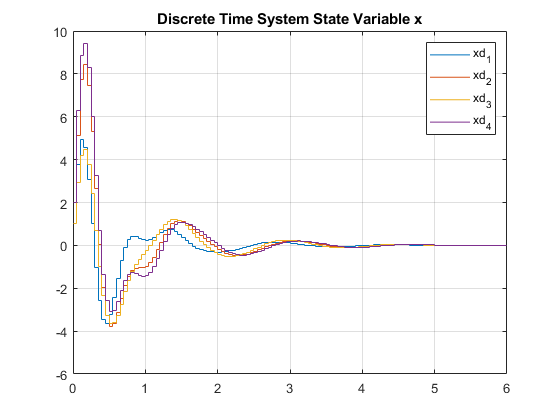
\includegraphics[width=\maxwidth{56.196688409433015em}]{figure_7.png}
\end{center}
\begin{matlabcode}
% Plot the output variable y
figure();
stairs(td,yd);
title("Discrete Time System Output Variable y");
xlim([0.00 6.00]);
ylim([-6.0 10.0]);
legend("yd_1", "yd_2");
grid on;
\end{matlabcode}
\begin{center}
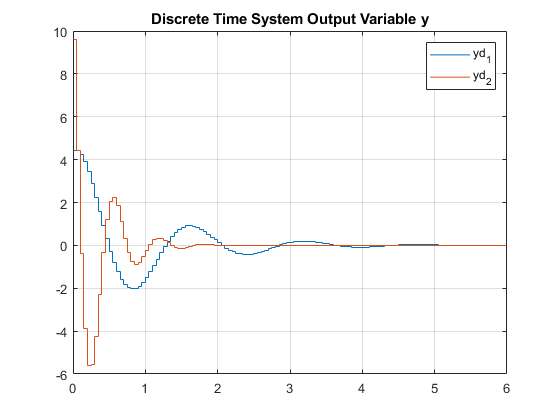
\includegraphics[width=\maxwidth{56.196688409433015em}]{figure_8.png}
\end{center}


\hrule
\matlabheadingthree{(e) }

\begin{par}
\begin{flushleft}
Vary the sampling period and describe the effect on the output. 
\end{flushleft}
\end{par}

\begin{matlabcode}
figure(1);
plot(t,y(:,1));
hold on

for ts = [0.2, 0.1, 0.05]
    td = 0:ts:10;
    ud = zeros(length(td), 2);
    sysd = c2d(sys, ts);
    
    [yd, td, xd] = lsim(sysd, ud, td, x_0);
    
    figure(1);
    stairs(td, yd(:,1));
end
hold off


figure(1);
title('Varied Sample Time of Discretised System');
xlim([0.00 3.00]);
ylim([-5.0 6.0]);
legend("continuous", "t_s = 0.2", "t_s = 0.1", "t_s = 0.05");
ylabel('y_1');
xlabel('t[s]');
grid on;
\end{matlabcode}
\begin{center}
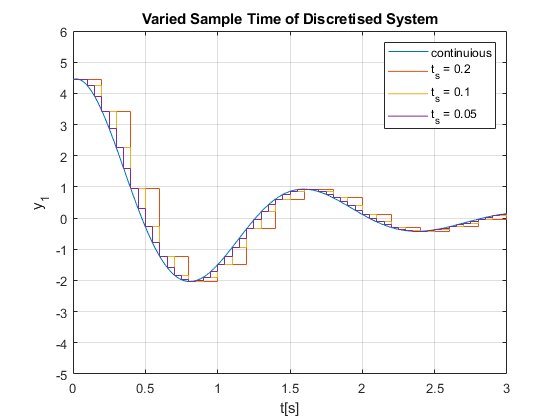
\includegraphics[width=\maxwidth{56.196688409433015em}]{figure_9.png}
\end{center}

\begin{par}
\begin{flushleft}
It can be seen that varying the the sampling period has a large affect on the output of the discretised system. As expected, increasing the sampling period of the signal will increase the accuracy of the discrete output. Because of this, it should be ensured that an adequate sampling time is selected to be able to properly represent the system.  
\end{flushleft}
\end{par}


\hrule
\matlabheadingthree{(f) }

\begin{par}
\begin{flushleft}
Find the time response for the discrete time system if there is no input and initial conditions of $\mathit{\mathbf{x}}={\left\lbrack 1\;\;\;\;1\;\;\;\;1\;\;\;\;2\right\rbrack }^T$ . Determine this response using powers of $\mathit{\mathbf{A}}$ directly (ie, do not use lsim). 
\end{flushleft}
\end{par}

\begin{matlabcode}
x_d = [];
y_d = [];

ts = 0.05;
td = 0:ts:10;
A_d = expm(ts*A);

for td_ = 0:ts:10
    xd = (A_d^(td_/ts))*x_0;
    yd = C*xd;
    
    x_d = [x_d; real(xd)'];
    y_d = [y_d; real(yd)'];
end

figure();
stairs(td, y_d)
hold on
stairs(t, y);
xlim([0.00 3.00]);
ylim([-6.0 10.0]);
title('Discretised System using powers of A');
legend("Discrete y_1", "Discrete y_2", "Continuious y_1", "Continuious y_2");
xlabel('t[s]');
hold off
\end{matlabcode}
\begin{center}
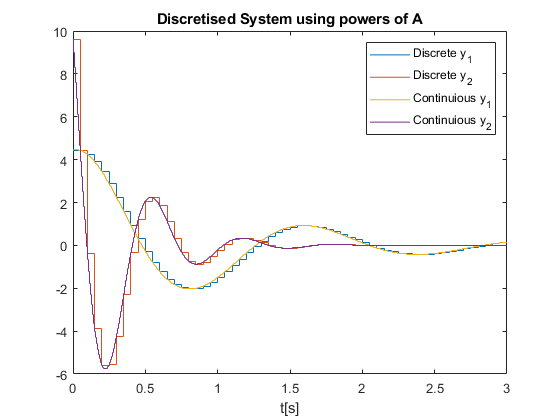
\includegraphics[width=\maxwidth{56.196688409433015em}]{figure_10.png}
\end{center}


\hrule
\matlabheadingtwo{Question 2}
\hrule\vspace{15pt}

\begin{par}
\begin{flushleft}
The phase-shift oscillator circuit shown in figure 1 can be described by the coupled differential equations
\end{flushleft}
\end{par}

\begin{par}
$$\begin{array}{l}
{\dot{v} }_a =-\frac{2v_a }{\textrm{RC}}+\frac{v_b }{\textrm{RC}}-\frac{R_2 }{R_1 }\frac{v_c }{\textrm{RC}}\\
{\dot{v} }_b =\frac{v_a }{\textrm{RC}}-\frac{2v_b }{\textrm{RC}}+\frac{v_c }{\textrm{RC}}\\
{\dot{v} }_c =\frac{v_b }{\textrm{RC}}-\frac{v_c }{\textrm{RC}}-\frac{v_c }{R_1 C}
\end{array}$$
\end{par}

\begin{par}
\begin{flushleft}
where $v_a$, $v_b$ and $v_c$ are the voltages after the three successive $\textrm{RC}$ stages.
\end{flushleft}
\end{par}

\begin{par}
\begin{center}
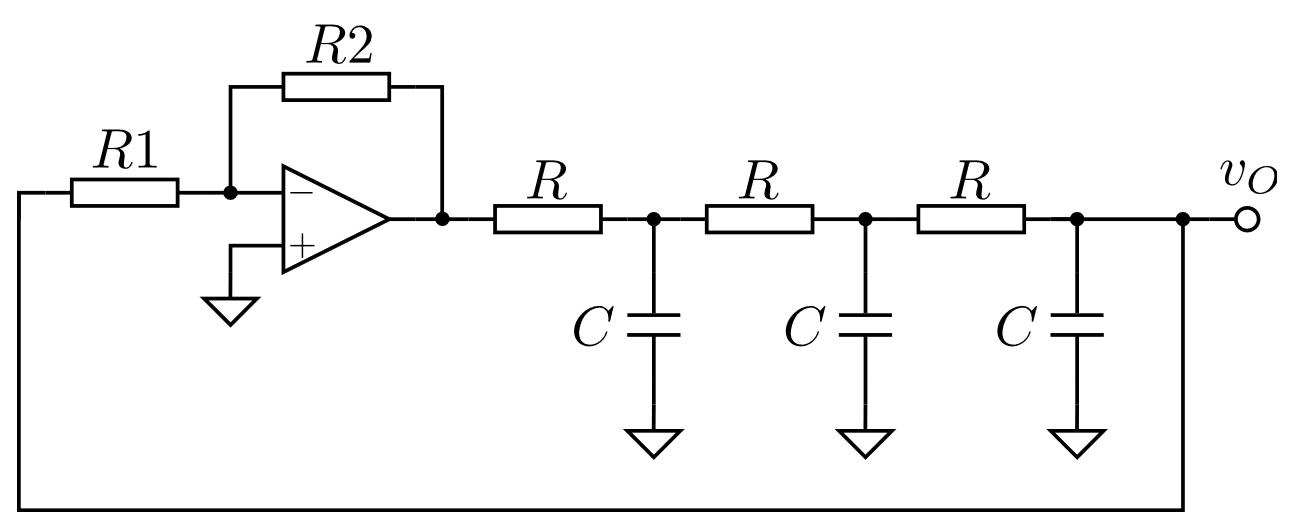
\includegraphics[width=\maxwidth{61.01354741595585em}]{image_0}
\end{center}
\end{par}

\begin{par}
\begin{center}
Figure 1: An unbuffered phase-shift oscillator
\end{center}
\end{par}


\vspace{1em}

\hrule
\matlabheadingthree{\textbf{(a) }\textit{Write a state space representation for the system.}}

\begin{par}
$$\left\lbrack \begin{array}{c}
{\dot{v} }_a \\
{\dot{v} }_b \\
{\dot{v} }_c 
\end{array}\right\rbrack =\left\lbrack \begin{array}{ccc}
-\frac{2}{\textrm{RC}} & \frac{1}{\textrm{RC}} & -\frac{R_2 }{R_1 }\frac{1}{\textrm{RC}}\\
\frac{1}{\textrm{RC}} & -\frac{2}{\textrm{RC}} & \frac{1}{\textrm{RC}}\\
0 & \frac{1}{\textrm{RC}} & -\left(\frac{1}{\textrm{RC}}+\frac{1}{R_1 C}\right)
\end{array}\right\rbrack \left\lbrack \begin{array}{c}
v_a \\
v_b \\
v_c 
\end{array}\right\rbrack$$
\end{par}


\vspace{1em}
\begin{par}
$$v_o = \left\lbrack \begin{array}{ccc}
0 & 0 & 1
\end{array}\right\rbrack \left\lbrack \begin{array}{c}
v_a \\
v_b \\
v_c 
\end{array}\right\rbrack$$
\end{par}


\vspace{1em}
\begin{par}
$$A=\left\lbrack \begin{array}{ccc}
-\frac{2}{\textrm{RC}} & \frac{1}{\textrm{RC}} & -\frac{R_2 }{R_1 }\frac{1}{\textrm{RC}}\\
\frac{1}{\textrm{RC}} & -\frac{2}{\textrm{RC}} & \frac{1}{\textrm{RC}}\\
0 & \frac{1}{\textrm{RC}} & -\left(\frac{1}{\textrm{RC}}+\frac{1}{R_1 C}\right)
\end{array}\right\rbrack ,\;\;\;C=\left\lbrack \begin{array}{ccc}
0 & 0 & 1
\end{array}\right\rbrack$$
\end{par}

\vspace{15pt}
\hrule
\matlabheadingthree{\textbf{(b) }\textit{The ratio }$\frac{\textrm{R2}}{\textrm{R1}}\approx 30$\textit{ matters if the oscillator is to maintain sustained oscillations.}}

\begin{par}
\begin{flushleft}
\textit{Find the value for this ratio that correctly induces oscillation, making sure that you explain your process.}
\end{flushleft}
\end{par}

\begin{par}
\begin{flushleft}
\textit{Hint: You could solve this problem analytically, but don’t!}
\end{flushleft}
\end{par}

\begin{par}
\begin{flushleft}
\textit{Hint: You should choose some convenient values for R and C, given that the nominal oscillation angular frequency is }$\omega_0 =\frac{1}{\sqrt{6}\textrm{RC}}$\textit{ .}
\end{flushleft}
\end{par}


\vspace{1em}
\begin{par}
\begin{flushleft}
For a system to maintain oscillation, it's most dominant poles but be a complex conjugate pair with no real real components (placed on the imaginary axis). Using this information, we are able to find a ratio of $\frac{\textrm{R2}}{\textrm{R1}}$ that will dive us sustained oscillation by varying the value of $\textrm{R2}$ and observing the poles of the system. 
\end{flushleft}
\end{par}

\begin{par}
\begin{flushleft}
For a state space system the eigenvalues of the $A$ matrix correspond to its poles. By looping through a range of $\textrm{R2}$ values and looking at the $A$matrix eigenvalues, we can look for a conjugate pair with no real component.
\end{flushleft}
\end{par}

\begin{par}
\begin{flushleft}
All calculations for this question have been done using $R=R_1 =1000$.
\end{flushleft}
\end{par}

\begin{matlabcode}
clc;
clear;

R = 1000;
R_1 = R;
c = 1e-3;

B = [];
C = [0, 0, 1];
D = [];

reals = [];
r = [];
r_oscillation = 0;

for R_2 = R:100:100*R
    
    % Calculate the A matrix
    A = [(-2/(R*c)), 1/(R*c), (-R_2/R_1)*(1/(R*c));
         1/(R*c),(-2/(R*c)),  1/(R*c);
         0, 1/(R*c), -(1/(R*c) + 1/(R_1*c))];
    
    % Store the real component of one of the complex pair eigenvalues
    reals = [reals; abs(real(eig(A)))'];
    r = [r; R_2];
    
    % Check if this real component is zero
    if reals(end, 2) == 0
        oscillation_ratio = R_2/R_1;
    end
end

figure();
plot(r, reals(:,2), '*-','MarkerEdgeColor','red','MarkerIndices',(oscillation_ratio*R_1-R)/100)
title("Real component of eigenvalues vs R_2")

text(47000,0.15,"R_2 = 56000");
text(55000,0.1,"\downarrow");

xlabel('R_2')
ylabel('|Re (\lambda_2)|')
\end{matlabcode}
\begin{center}
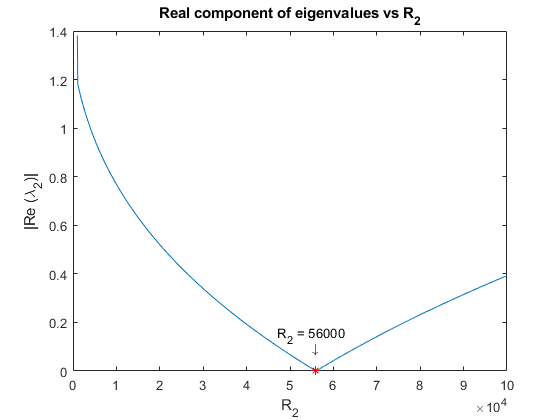
\includegraphics[width=\maxwidth{56.196688409433015em}]{figure_11.png}
\end{center}

\begin{par}
\begin{flushleft}
The plot above displays how the real component of $\lambda_2$ behaves as we increase $R_2$. From this it can be seen that at an $R_2$ value of $56000$ will provide sustained oscillation. This gives us a final ratio of $\frac{\textrm{R2}}{\textrm{R1}}=56$.
\end{flushleft}
\end{par}


\matlabheadingthree{\textbf{(c) }\textit{Determine the oscillation frequency of the circuit using the state space model.}}

\begin{par}
\hfill \break
\end{par}

\begin{matlabcode}
R_2 = oscillation_ratio*R;

A = [(-2/(R*c)), 1/(R*c), (-R_2/R_1)*(1/(R*c));
     1/(R*c),(-2/(R*c)),  1/(R*c);
     0, 1/(R*c), -(1/(R*c) + 1/(R_1*c))];
 
sys_poles = eig(A);

f_s = imag(sys_poles(2))/(2*pi)
\end{matlabcode}
\begin{matlaboutput}
f_s = 0.5033
\end{matlaboutput}

\begin{par}
\begin{flushleft}
The oscillation frequency of this circuit is $0\ldotp 5033\;\textrm{Hz}$
\end{flushleft}
\end{par}


\vspace{1em}
\matlabheadingthree{\textbf{(d) }\textit{Simulate the operation of the oscillator to show that it works as you might expect.}}

\begin{par}
\begin{flushleft}
\textit{Hint: Think about the initial conditions for the simulation.}
\end{flushleft}
\end{par}

\begin{matlabcode}
sys = ss(A, B, C, D);

[V, wc] = eig(A);
x_0 = V(:, 2);

t = 0:f_s/100:5/f_s;

[y, t, x] = lsim(sys, [], t, x_0);

figure();
plot(t,real(x));
title("System State Variables");
legend("v_a","v_b","v_c");
xlabel('t[s]')
ylabel('V(s)')
grid on;
\end{matlabcode}
\begin{center}
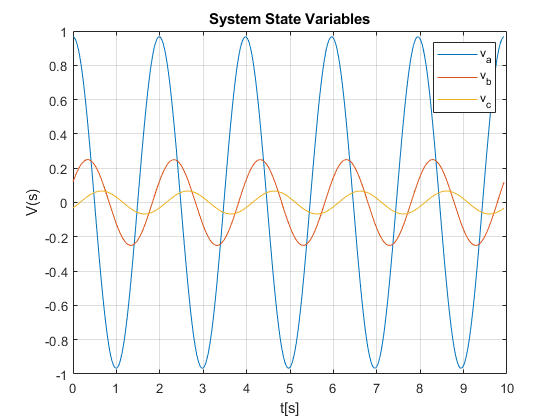
\includegraphics[width=\maxwidth{56.196688409433015em}]{figure_12.png}
\end{center}
\begin{matlabcode}
figure();
plot(t,real(y));
title("Output");
legend("v_o");
xlabel('t[s]')
ylabel('V(s)')
grid on;
\end{matlabcode}
\begin{center}
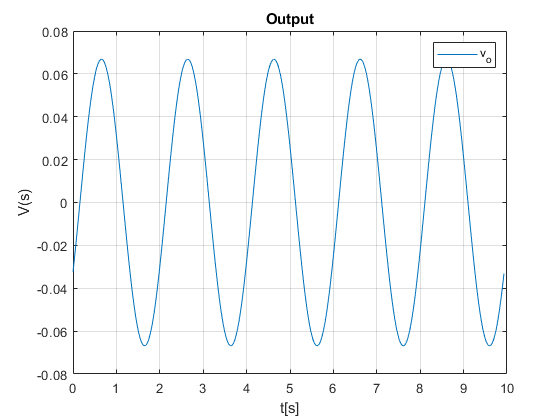
\includegraphics[width=\maxwidth{56.196688409433015em}]{figure_13.png}
\end{center}

\hrule\vspace{20pt}
\matlabheading{Section B - Summative Questions}
\hrule\vspace{20pt}


\matlabheadingthree{\textit{You need to design a simple open loop "controller" that causes a rocket to pitch }${10}^{\circ }$\textit{ clockwise by the end of the first 15 seconds of flight. The idea is nominally to let the rocket ascend for the first five seconds and then pitch over at approximately }$1^{\circ } /s$\textit{ for the remaining 10 seconds. The main rocket engine is at full burn throughout the period.}}

\matlabheadingthree{\textit{A continuous time, nonlinear model for the rocket is as described below. Simulation code for the complete nonlinear system is available on the course website.}}

\matlabheadingthree{\textit{In this question you will investigate the approximations due to linearisation of the system, as well as examining the time evolution of the system.}}


\vspace{1em}
\begin{par}
\begin{flushleft}
Let the state vector be defined as follows:
\end{flushleft}
\end{par}

\begin{par}
\begin{flushleft}
                        $x_1 \equiv$ Rocket’s altitude (positive upwards) $\left\lbrack m\right\rbrack$
\end{flushleft}
\end{par}

\begin{par}
\begin{flushleft}
                        $x_2 \equiv$ Rocket’s vertical velocity (positive upwards) $m/s$
\end{flushleft}
\end{par}

\begin{par}
\begin{flushleft}
                        $x_3 \equiv$ Rocket’s horizontal position relative to launch site $\left\lbrack m\right\rbrack$
\end{flushleft}
\end{par}

\begin{par}
\begin{flushleft}
                        $x_4 \equiv$ Rocket’s horizontal ground speed $\left\lbrack m/s\right\rbrack$
\end{flushleft}
\end{par}

\begin{par}
\begin{flushleft}
                        $x_5 \equiv$ Rocket’s angle from vertical $\left\lbrack \circ \right\rbrack$
\end{flushleft}
\end{par}

\begin{par}
\begin{flushleft}
                        $x_6 \equiv$ Rocket’s angular velocity $\left\lbrack \circ /s\right\rbrack$
\end{flushleft}
\end{par}

\begin{par}
\begin{flushleft}
                        $x_7 \equiv$ Fuel load $\left\lbrack \textrm{kg}\right\rbrack$
\end{flushleft}
\end{par}

\begin{par}
\begin{flushleft}
and the input vector is:
\end{flushleft}
\end{par}

\begin{par}
\begin{flushleft}
                        $u_1 \equiv$ Main engine force (positive upwards) $\left\lbrack N\right\rbrack$
\end{flushleft}
\end{par}

\begin{par}
\begin{flushleft}
                        $u_2 \equiv$ Orientation thruster force (positive rotates the rocket clockwise) $\left\lbrack N\right\rbrack$
\end{flushleft}
\end{par}

\begin{par}
\begin{flushleft}
The initial state is:
\end{flushleft}
\end{par}

\begin{par}
\begin{flushleft}
                        $x\left(0\right)={\left\lbrack \begin{array}{ccccccc}
0 & 0 & 0 & 0 & 0 & 0 & 1000
\end{array}\right\rbrack }^T$,
\end{flushleft}
\end{par}

\begin{par}
\begin{flushleft}
which is to say that before launch it is stationary at the origin, with 1000 kg of fuel on board.
\end{flushleft}
\end{par}

\begin{par}
\begin{flushleft}
The rocket’s state evolves according to the following set of nonlinear equations.
\end{flushleft}
\end{par}

\begin{par}
$$\left\lbrace \begin{array}{l}
{\dot{x} }_1 =x_2 \\
{\dot{x} }_2 =g-c_d x_2^2 +\frac{\mathrm{cos}\left(x_5 \right)}{\left(M+x_7 \right)}u_1 \\
{\dot{x} }_3 =x_4 \\
{\dot{x} }_4 =-\frac{\mathrm{sin}\left(x_5 \right)}{\left(M+x_7 \right)}u_1 \\
{\dot{x} }_5 =x_6 \\
{\dot{x} }_6 =\frac{k}{J+L^2 x_7 }\\
{\dot{x} }_7 =-\frac{1}{\eta }\left(u_1 +u_2 \right)
\end{array}\right.$$
\end{par}

\begin{par}
\begin{center}
where,$\left\lbrace \begin{array}{l}
g=9\ldotp 8\;\mathrm{the}\;\mathrm{acceleration}\;\mathrm{due}\;\mathrm{to}\;\mathrm{gravity}\;\left\lbrack {\mathrm{ms}}^{-2} \right\rbrack \\
c_d =2\times {10}^{-3} \;\mathrm{is}\;\mathrm{the}\;\mathrm{coefficient}\;\mathrm{of}\;\mathrm{drag}\;\left\lbrack {\mathrm{Nm}}^{-2} s^2 \right\rbrack \\
M=1000\;\mathrm{is}\;\mathrm{the}\;\mathrm{mass}\;\mathrm{of}\;\mathrm{the}\;\mathrm{empty}\;\mathrm{rocket}\;\left\lbrack \mathrm{kg}\right\rbrack \\
J=20,000\;\mathrm{is}\;\mathrm{the}\;\mathrm{moment}\;\mathrm{of}\;\mathrm{inertia}\;\mathrm{of}\;\mathrm{empty}\;\mathrm{rocket}\;\left\lbrack \mathrm{kg}\;m^2 \right\rbrack \\
L=5\;\mathrm{is}\;\mathrm{the}\;\mathrm{distance}\;\mathrm{between}\;\mathrm{the}\;\mathrm{rockets}\;\mathrm{centre}\;\mathrm{of}\;\mathrm{mass}\;\mathrm{and}\;\mathrm{the}\;\\ \hspace{20pt}\mathrm{centre}\;\mathrm{of}\;\mathrm{the}\;\mathrm{fuel}\;\mathrm{load}\;\left\lbrack m\right\rbrack \\
\eta =1000\;\mathrm{is}\;\mathrm{the}\;\mathrm{efficiency}\;\mathrm{of}\;\mathrm{the}\;\mathrm{fuel}\;\left\lbrack \mathrm{Ns}/\mathrm{kg}\right\rbrack \\
k=6\;\mathrm{is}\;\mathrm{the}\;\mathrm{distance}\;\mathrm{between}\;\mathrm{the}\;\mathrm{rotation}\;\mathrm{thruster}\;\mathrm{and}\;\mathrm{the}\;\mathrm{centre}\;\mathrm{of}\;\\\hspace{20pt} \mathrm{mass}\;\left\lbrack \mathrm{Ns}/\mathrm{kg}\right\rbrack 
\end{array}\right.$
\end{center}
\end{par}

\begin{par}
\begin{flushleft}
(Note that these quantities may not make physical sense; they are constructed to make an interesting exercise. In addition, the model doesn’t attempt to capture all of the nonlinear effects. As an example $L$ should most likely change as the fuel load is depleted.)
\end{flushleft}
\end{par}

\begin{par}
\begin{flushleft}
Hints:
\end{flushleft}
\end{par}

\begin{par}
\begin{flushleft}
1. The nonlinear simulation code calculates the rocket’s trajectory in time chunks of length \texttt{\textbf{dt}}. The control input $\mathit{\mathbf{u}}$ is calculated only once per time chunk. If you decrease \texttt{\textbf{dt}}\texttt{ }the ODE solver may be more accurate, and as a side effect you can calculate $\mathit{\mathbf{u}}$ more frequently (and vice versa). This may be useful for debugging, but your final solution will be marked with \texttt{\textbf{dt=1}}. However, for this assignment you need not change $\mathit{\mathbf{u}}$ anyway, so there is little to be gained by changing $\textrm{dt}$.
\end{flushleft}
\end{par}

\begin{par}
\begin{flushleft}
2. The sample code includes a symbolic model \texttt{\textbf{f\_sym}}\texttt{ }that should be useful in finding the linear approximations of the system, but you may choose to find it by hand. To implement the linearized systems, you should find a linear model and then rewrite the simulation section of the code to use \texttt{\textbf{lsim}}\texttt{ }rather than \texttt{\textbf{ode45}}.
\end{flushleft}
\end{par}


\begin{par}
\begin{flushleft}

\hrule\vspace{20pt}
\textbf{a)} \textbf{[5 marks]}\textit{ Use the nonlinear model to devise a nominal control signal }$\mathit{\mathbf{u}}$\textit{. You should assume that }$u_1$\textit{ is a constant throughout the 15 seconds of flight, such that there is no remaining fuel after that time. You should then choose }$u_2$\textit{ to effect the required pitch-over manoeuvre.}
\end{flushleft}
\end{par}

\begin{par}
\begin{flushleft}
\textit{You don’t need to be too fussy about this; just devise something simple that you can use for comparison in the following parts of the question.}
\end{flushleft}
\end{par}

\begin{par}
\begin{flushleft}
\textit{Hint: Your code to set }$\mathit{\mathbf{u}}$\textit{ should go in the section marked with asterisks. The simulation will not do much until you put something in this section.}
\end{flushleft}
\end{par}


\vspace{1em}
\begin{par}
\begin{flushleft}
Ans. $\left\lbrack \begin{array}{c}
u_1 \\
u_2 
\end{array}\right\rbrack =\left\lbrack \begin{array}{c}
50040\\
1140
\end{array}\right\rbrack \to \textrm{final}\;\textrm{angle}:10\ldotp {0000}^{\circ }$
\end{flushleft}
\end{par}

\begin{matlabcode}
clc;
clear;
run("Assignment_2_2021_Q3_a.m");
\end{matlabcode}
\begin{center}
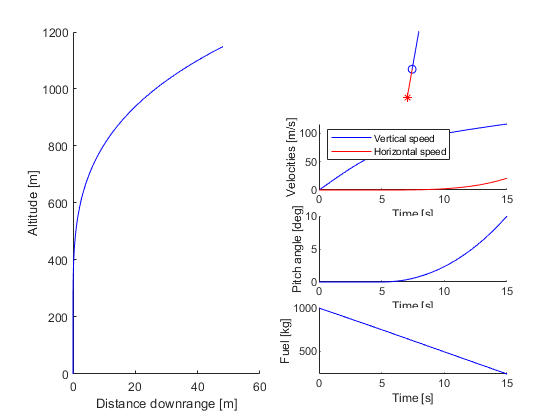
\includegraphics[width=\maxwidth{56.196688409433015em}]{figure_14.png}
\end{center}
\begin{matlaboutput}
final_angle = 10.0000
\end{matlaboutput}


\begin{par}
\begin{flushleft}
\hrule\vspace{20pt}
\textbf{b) [2 marks]} \textit{What is the maximum acceleration seen by the rocket during the launch?}
\end{flushleft}
\end{par}

\begin{matlabcode}
% % Clean the data to remove the double ups
t_store = unique(t_store);
x_store = unique(x_store,"rows");

% % Store the vertical and horizontal velocity
v_y = x_store(:, 2);
v_x = x_store(:, 4);

% % Take a numerical derivative
a_y = diff(v_y)./diff(t_store);
a_x = diff(v_x)./diff(t_store);

% % Calculate the Total acceleration (Combination of a_x and a_y)
a_total = sqrt((a_x.^2)+(a_y.^2));
[M,I] = max(a_total);

subplot(111);
plot(t_store(2:end), a_y, t_store(2:end), a_x, t_store(2:end), a_total, '.-','MarkerEdgeColor','red','MarkerIndices', I)
% plot(t_store(2:end), a_x)
% plot(t_store(2:end), a_total, '.-','MarkerEdgeColor','red','MarkerIndices', I)
title("Acceleration Plot")
legend('Vertical Acceleration', 'Horizontal Acceleration', 'Total Acceleration')
text(t_store(I-20), M-0.8, num2str(a_total(I)))
xlabel('t[s]')
ylabel('m/s^2')
\end{matlabcode}
\begin{center}
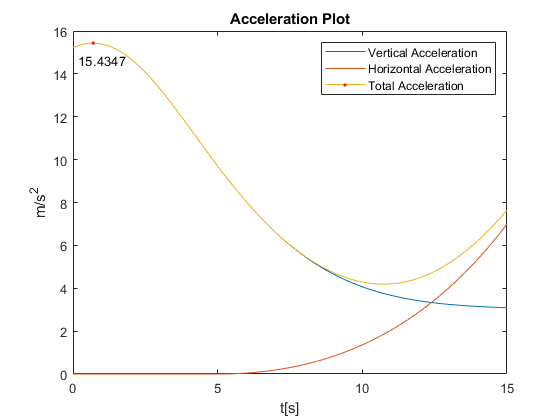
\includegraphics[width=\maxwidth{56.196688409433015em}]{figure_15.png}
\end{center}

\begin{par}
\begin{flushleft}
The maximum acceleration seen by the rocket during the launch is $15\ldotp 4347\;m$/$s^2$
\end{flushleft}
\end{par}


\begin{par}
\begin{flushleft}
\hrule\vspace{20pt}
\textbf{c) [3 marks] }\textit{Which state variables are important in the linearisation? That is, in which variables is the model nonlinear? Provide physical reasoning for the identified nonlinearities.}
\end{flushleft}
\end{par}

\begin{par}
\begin{flushleft}

By looking at the state vector descriptions we can see that $\dot{x_2 } \;,\;\dot{x_4 } \;,\;\dot{x_6 }$ are the accelerations of the rocket, as they are the derivatives of the rocket velocities. We know that the acceleration of the rocket will be inherently non-linear, as the mass of the rocket is changing thought the flight, and the drag coefficient of the rocket will also not remain constant. We can also see from the acceleration plot above that all these accelerations are non-constant, and therefore are non-linear. 

From this we can say that the velocities $x_2 \;,\;x_4 \;,x_6 \;$are also all non-constant, as they are the integrals of $\dot{x_2 } \;,\;\dot{x_4 } \;,\;\dot{x_6 }$, and therefore non-linear. Finally we can see that $\dot{x_1 } \;,\;\dot{x_3 } \;,\;\dot{x_{5\;\;} }$are all derived from $x_2 \;,\;x_4 \;,x_6$ and therefore these state variables will also be non-linear.

\end{flushleft}
\end{par}

\begin{par}
\begin{flushleft}
The means that the only linear state variable within this model is $x_7 \ldotp$
\end{flushleft}
\end{par}


\begin{par}
\begin{flushleft}
\hrule\vspace{20pt}
\textbf{d) [5 marks] }\textit{Linearize the model at the position where it begins its pitch-over manoeuvre }$\left(t=5\right)$\textit{ and plot the rocket’s trajectory when you apply your nominal control signal.}
\end{flushleft}
\end{par}

\begin{matlabcode}
u1_const = 50040;
opp_point = 5;

syms u1 u2

Df_x = jacobian(f_sym, [x1 x2 x3 x4 x5 x6 x7])
\end{matlabcode}
\begin{matlabsymbolicoutput}
Df_x = 

\hskip1em $\displaystyle \left(\begin{array}{ccccccc}
0 & 1 & 0 & 0 & 0 & 0 & 0\\
0 & -\frac{x_2 }{250} & 0 & 0 & -\frac{u_1 \,\sin \left(x_5 \right)}{x_7 +1000} & 0 & -\frac{u_1 \,\cos \left(x_5 \right)}{{{\left(x_7 +1000\right)}}^2 }\\
0 & 0 & 0 & 1 & 0 & 0 & 0\\
0 & 0 & 0 & 0 & \frac{u_1 \,\cos \left(x_5 \right)}{x_7 +1000} & 0 & -\frac{u_1 \,\sin \left(x_5 \right)}{{{\left(x_7 +1000\right)}}^2 }\\
0 & 0 & 0 & 0 & 0 & 1 & 0\\
0 & 0 & 0 & 0 & 0 & 0 & -\frac{150\,u_2 }{{{\left(25\,x_7 +20000\right)}}^2 }\\
0 & 0 & 0 & 0 & 0 & 0 & 0
\end{array}\right)$
\end{matlabsymbolicoutput}
\begin{matlabcode}
A = subs(Df_x, [x1 x2 x3 x4 x5 x6 x7 u1 u2], 
     [x_store(t_store==opp_point,:), u1_const, 0])
\end{matlabcode}
\begin{matlabsymbolicoutput}
A = 

\hskip1em $\displaystyle \left(\begin{array}{ccccccc}
0 & 1 & 0 & 0 & 0 & 0 & 0\\
0 & -\frac{1187950448851753}{4398046511104000} & 0 & 0 & 0 & 0 & -\frac{1251000}{76545001}\\
0 & 0 & 0 & 1 & 0 & 0 & 0\\
0 & 0 & 0 & 0 & \frac{250200}{8749} & 0 & 0\\
0 & 0 & 0 & 0 & 0 & 1 & 0\\
0 & 0 & 0 & 0 & 0 & 0 & 0\\
0 & 0 & 0 & 0 & 0 & 0 & 0
\end{array}\right)$
\end{matlabsymbolicoutput}
\begin{matlabcode}
A = double(A);

Df_u = jacobian(f_sym, [u1 u2])
\end{matlabcode}
\begin{matlabsymbolicoutput}
Df_u = 

\hskip1em $\displaystyle \left(\begin{array}{cc}
0 & 0\\
\frac{\cos \left(x_5 \right)}{x_7 +1000} & 0\\
0 & 0\\
\frac{\sin \left(x_5 \right)}{x_7 +1000} & 0\\
0 & 0\\
0 & \frac{6}{25\,x_7 +20000}\\
-\frac{1}{1000} & -\frac{1}{1000}
\end{array}\right)$
\end{matlabsymbolicoutput}
\begin{matlabcode}
B = subs(Df_u, [x1 x2 x3 x4 x5 x6 x7 u1 u2], 
     [x_store(t_store==opp_point,:), u1_const, 0])
\end{matlabcode}
\begin{matlabsymbolicoutput}
B = 

\hskip1em $\displaystyle \left(\begin{array}{cc}
0 & 0\\
\frac{5}{8749} & 0\\
0 & 0\\
0 & 0\\
0 & 0\\
0 & \frac{2}{12915}\\
-\frac{1}{1000} & -\frac{1}{1000}
\end{array}\right)$
\end{matlabsymbolicoutput}
\begin{matlabcode}
B = double(B);

sys = ss(A, B, [], []);
figure();
run("Assignment_2_2021_Q3_linear.m");
\end{matlabcode}
\begin{center}
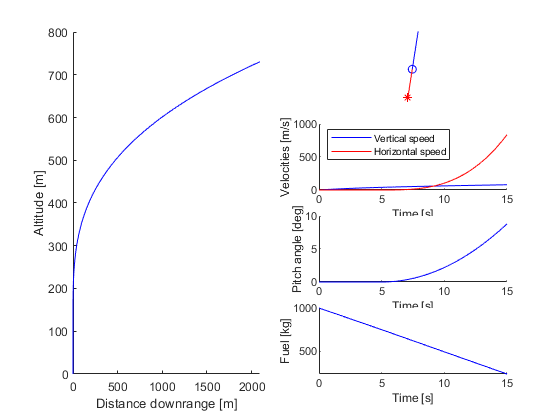
\includegraphics[width=\maxwidth{56.196688409433015em}]{figure_16.png}
\end{center}
\begin{matlabcode}
final_angle = x(end,5)
\end{matlabcode}
\begin{matlaboutput}
final_angle = 8.8093
\end{matlaboutput}


\begin{par}
\begin{flushleft}
\textbf{e) [5 marks]}\textit{\textbf{ }}\textit{Linearize the model at its final position }$\left(t=15\right)$\textit{ and plot the rocket trajectory when you apply your nominal control signal.}
\end{flushleft}
\end{par}

\begin{matlabcode}
u1_const = 50040;
opp_point = 15;

syms u1 u2

Df_x = jacobian(f_sym, [x1 x2 x3 x4 x5 x6 x7])
\end{matlabcode}
\begin{matlabsymbolicoutput}
Df_x = 

\hskip1em $\displaystyle \left(\begin{array}{ccccccc}
0 & 1 & 0 & 0 & 0 & 0 & 0\\
0 & -\frac{x_2 }{250} & 0 & 0 & -\frac{u_1 \,\sin \left(x_5 \right)}{x_7 +1000} & 0 & -\frac{u_1 \,\cos \left(x_5 \right)}{{{\left(x_7 +1000\right)}}^2 }\\
0 & 0 & 0 & 1 & 0 & 0 & 0\\
0 & 0 & 0 & 0 & \frac{u_1 \,\cos \left(x_5 \right)}{x_7 +1000} & 0 & -\frac{u_1 \,\sin \left(x_5 \right)}{{{\left(x_7 +1000\right)}}^2 }\\
0 & 0 & 0 & 0 & 0 & 1 & 0\\
0 & 0 & 0 & 0 & 0 & 0 & -\frac{150\,u_2 }{{{\left(25\,x_7 +20000\right)}}^2 }\\
0 & 0 & 0 & 0 & 0 & 0 & 0
\end{array}\right)$
\end{matlabsymbolicoutput}
\begin{matlabcode}
A = subs(Df_x, [x1 x2 x3 x4 x5 x6 x7 u1 u2], 
          [x_store(t_store==opp_point,:), u1_const, 0])
\end{matlabcode}
\begin{matlabsymbolicoutput}
A = 

\hskip1em $\displaystyle \left(\begin{array}{ccccccc}
0 & 1 & 0 & 0 & 0 & 0 & 0\\
0 & -\frac{2040878444777219}{4398046511104000} & 0 & 0 & -\frac{25020\,\sin \left(\frac{5629518589717605}{562949953421312}\right)}{619} & 0 & -\frac{12510\,\cos \left(\frac{5629518589717605}{562949953421312}\right)}{383161}\\
0 & 0 & 0 & 1 & 0 & 0 & 0\\
0 & 0 & 0 & 0 & \frac{25020\,\cos \left(\frac{5629518589717605}{562949953421312}\right)}{619} & 0 & -\frac{12510\,\sin \left(\frac{5629518589717605}{562949953421312}\right)}{383161}\\
0 & 0 & 0 & 0 & 0 & 1 & 0\\
0 & 0 & 0 & 0 & 0 & 0 & 0\\
0 & 0 & 0 & 0 & 0 & 0 & 0
\end{array}\right)$
\end{matlabsymbolicoutput}
\begin{matlabcode}
A = double(A);

Df_u = jacobian(f_sym, [u1 u2])
\end{matlabcode}
\begin{matlabsymbolicoutput}
Df_u = 

\hskip1em $\displaystyle \left(\begin{array}{cc}
0 & 0\\
\frac{\cos \left(x_5 \right)}{x_7 +1000} & 0\\
0 & 0\\
\frac{\sin \left(x_5 \right)}{x_7 +1000} & 0\\
0 & 0\\
0 & \frac{6}{25\,x_7 +20000}\\
-\frac{1}{1000} & -\frac{1}{1000}
\end{array}\right)$
\end{matlabsymbolicoutput}
\begin{matlabcode}
B = subs(Df_u, [x1 x2 x3 x4 x5 x6 x7 u1 u2], [x_store(t_store==opp_point,:), u1_const, 0])
\end{matlabcode}
\begin{matlabsymbolicoutput}
B = 

\hskip1em $\displaystyle \left(\begin{array}{cc}
0 & 0\\
\frac{\cos \left(\frac{5629518589717605}{562949953421312}\right)}{1238} & 0\\
0 & 0\\
\frac{\sin \left(\frac{5629518589717605}{562949953421312}\right)}{1238} & 0\\
0 & 0\\
0 & \frac{1}{4325}\\
-\frac{1}{1000} & -\frac{1}{1000}
\end{array}\right)$
\end{matlabsymbolicoutput}
\begin{matlabcode}
B = double(B);

sys = ss(A, B, [], []);
figure();
run("Assignment_2_2021_Q3_linear.m");
\end{matlabcode}
\begin{center}
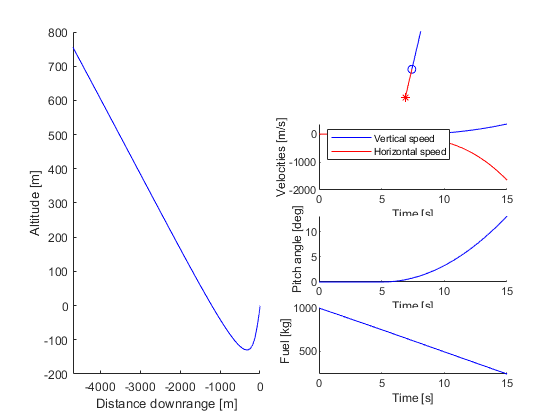
\includegraphics[width=\maxwidth{56.196688409433015em}]{figure_17.png}
\end{center}
\begin{matlabcode}
final_angle = x(end,5)
\end{matlabcode}
\begin{matlaboutput}
final_angle = 13.1528
\end{matlaboutput}


\begin{par}
\begin{flushleft}
\hrule\vspace{20pt}
\textbf{f) [5 marks] }\textit{Discuss what you have found from the linearisation, including the differences (if any) between them. What linearisation would you use in a practical implementation of this system?}\\ \vspace{20pt}

By comparing the two linearization's to the original simulation, we can see that neither perform well in predicting the models horizontal velocity or horizontal/vertical position (distance down range), however the prediction of the phase angle is not far from the original, and the fuel consumption is identical (since it was already linear). \vspace{10pt}

When comparing the linearisation around the operating point 't=5' to the linearisation around the operating point 't=15' we can see that there are drastic differences between these two models. For the model of 't=15', the horizontal velocity is negative rather than positive, and the magnitude of this velocity is far greater of that of the original. Because of this the horizontal position can be seen to be drastically incorrect. For the model of 't=5', the horizontal velocity has the correct sign, however the magnitude of this velocity is still far larger than the original system, leading to a much larger horizontal displacement.\vspace{10pt}

From this I would chose to use the linearization with the operation point of 't=5' as it provides the most accurate representation of the original system. However it should be noted that neither of the linear models provides an accurate representation of the original model. \vspace{10pt}

It should also be noted that when choosing an operating point for a linearisation, it is important to select the point to be either close to the middle of your simulation, or around a particular point of interest. This is because as your model moves further away from your operating point, there will be a greater error within your model.

\end{flushleft}
\end{par}

\end{preview}
\end{document}
